\documentclass[17pt, aspectratio=169]{beamer}

\beamertemplatenavigationsymbolsempty
\usetheme{CambridgeUS}
\usecolortheme{dolphin}
\useinnertheme{rectangles}
\usepackage{array}
\usepackage[subpreambles=true]{standalone}
\usepackage{import}


\title{M.O.S.I.S Final Report Presentation}
\author[Fabio J. \& Eduardo S.]{Fabio J. Matos Nieves \& Eduardo S. Miranda Figueroa}
\institute[UPRM]{University of Puerto Rico Mayagüez Campus}
\date{December 11, 2023}

\begin{document}
\begin{frame}
	\maketitle
\end{frame}
\begin{frame}
	\tableofcontents
\end{frame}
\section{Introduction}
\subsection*{Background}
\begin{frame}{What is M.O.S.I.S?}
	\begin{columns}
		\column{0.5\textwidth}
		\centering
		\textbf{M.O.S.I.S}\\
		Marine Operated Stereoscopic Imaging System

		\column{0.5\textwidth}
		\centering
		\begin{figure}
			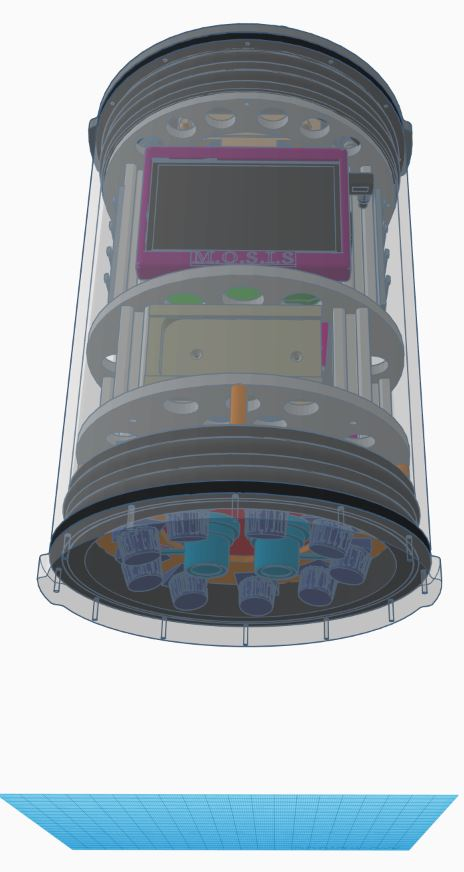
\includegraphics[height=0.85\textheight]{./Figures/M.O.S.I.S_Model.jpeg}
		\end{figure}
	\end{columns}
\end{frame}
\begin{frame}{What is the problem?}
	\begin{itemize}
		\item The M.O.S.I.S microscope already has a user interface \textbf{but}:
		      \begin{itemize}
			      \item lacks design cohesion.
			      \item has missing and redundant features.
			      \item constantly crashes.
			      \item lacks a formal way to store data.
		      \end{itemize}
	\end{itemize}
\end{frame}
\section{Body}
\subsection*{Design Alternatives}
\begin{frame}{Design Alternatives}
	\begin{itemize}

		\item There are three main architectural patterns used to create user interfaces
		      \begin{enumerate}
			      \item Web based
			      \item Native
			      \item Web-Native
		      \end{enumerate}
	\end{itemize}
\end{frame}
\subsection*{System Specifications}
\begin{frame}{System Specifications}
	\begin{itemize}
		\item 400\times400 preview for left and right cameras
		\item Displays temperature, pressure, dissolved oxygen and pH of the environment
		\item User interface navigation using on board buttons
		\item Controls camera parameters and on board lighting
		\item Calibrates pH and dissolved oxygen sensors
		\item Written in Python using PyQt6 and SQLite3
	\end{itemize}
\end{frame}
\subsection*{Validation and Testing}
\begin{frame}{Validation}
	\begin{enumerate}
		\item Thorough review of the system requirements
		\item Constant feedback from the client and stakeholder
	\end{enumerate}
\end{frame}
\begin{frame}{Testing}
	\begin{enumerate}
		\item Module Testing
		\item Integration Testing
		\item End to end testing
	\end{enumerate}
\end{frame}
\subsection*{Diagrams}\begin{frame}{M.O.S.I.S UI 2.0: System Architecture}
	\begin{figure}
		\resizebox{0.9\textwidth}{!}{
			\begin{small}
				\import{./Figures}{system_architecture}
			\end{small}
		}
		\caption{System Architecture}
	\end{figure}
\end{frame}
\subsection{Video Demo}
\subsection*{Deliverables and Milestones}
\subsection{Project Assessment}
\subsection*{Project Impact}
\subsection*{Expenditure Summary}
\begin{frame}{Expenditure Summary}
	\begin{center}
		\begin{tabular}{||m{0.75\textwidth} | m{0.20\textwidth} ||}
			\hline
			Eduardo S. Miranda \& Fabio J. Matos's Salary & \$18,430.61 \\
			\hline
			Facility Cost                                 & \$1,410.00  \\
			\hline
			Udemy PyQt6 Class                             & \$28.98     \\
			\hline
			Other benefits and overhead                   & \$21,832.84 \\
			\hline
			Total Budget Cost                             & \$41,703.03 \\
			\hline
		\end{tabular}
	\end{center}
\end{frame}
\section{Conclusion}
\subsection{Deliverables}
\subsection{Achievements and Lessons Learned}
\end{document}